\subsection{Standard Model W$\gamma$ Production}

\begin{figure}[htb]
  \begin{center}
    {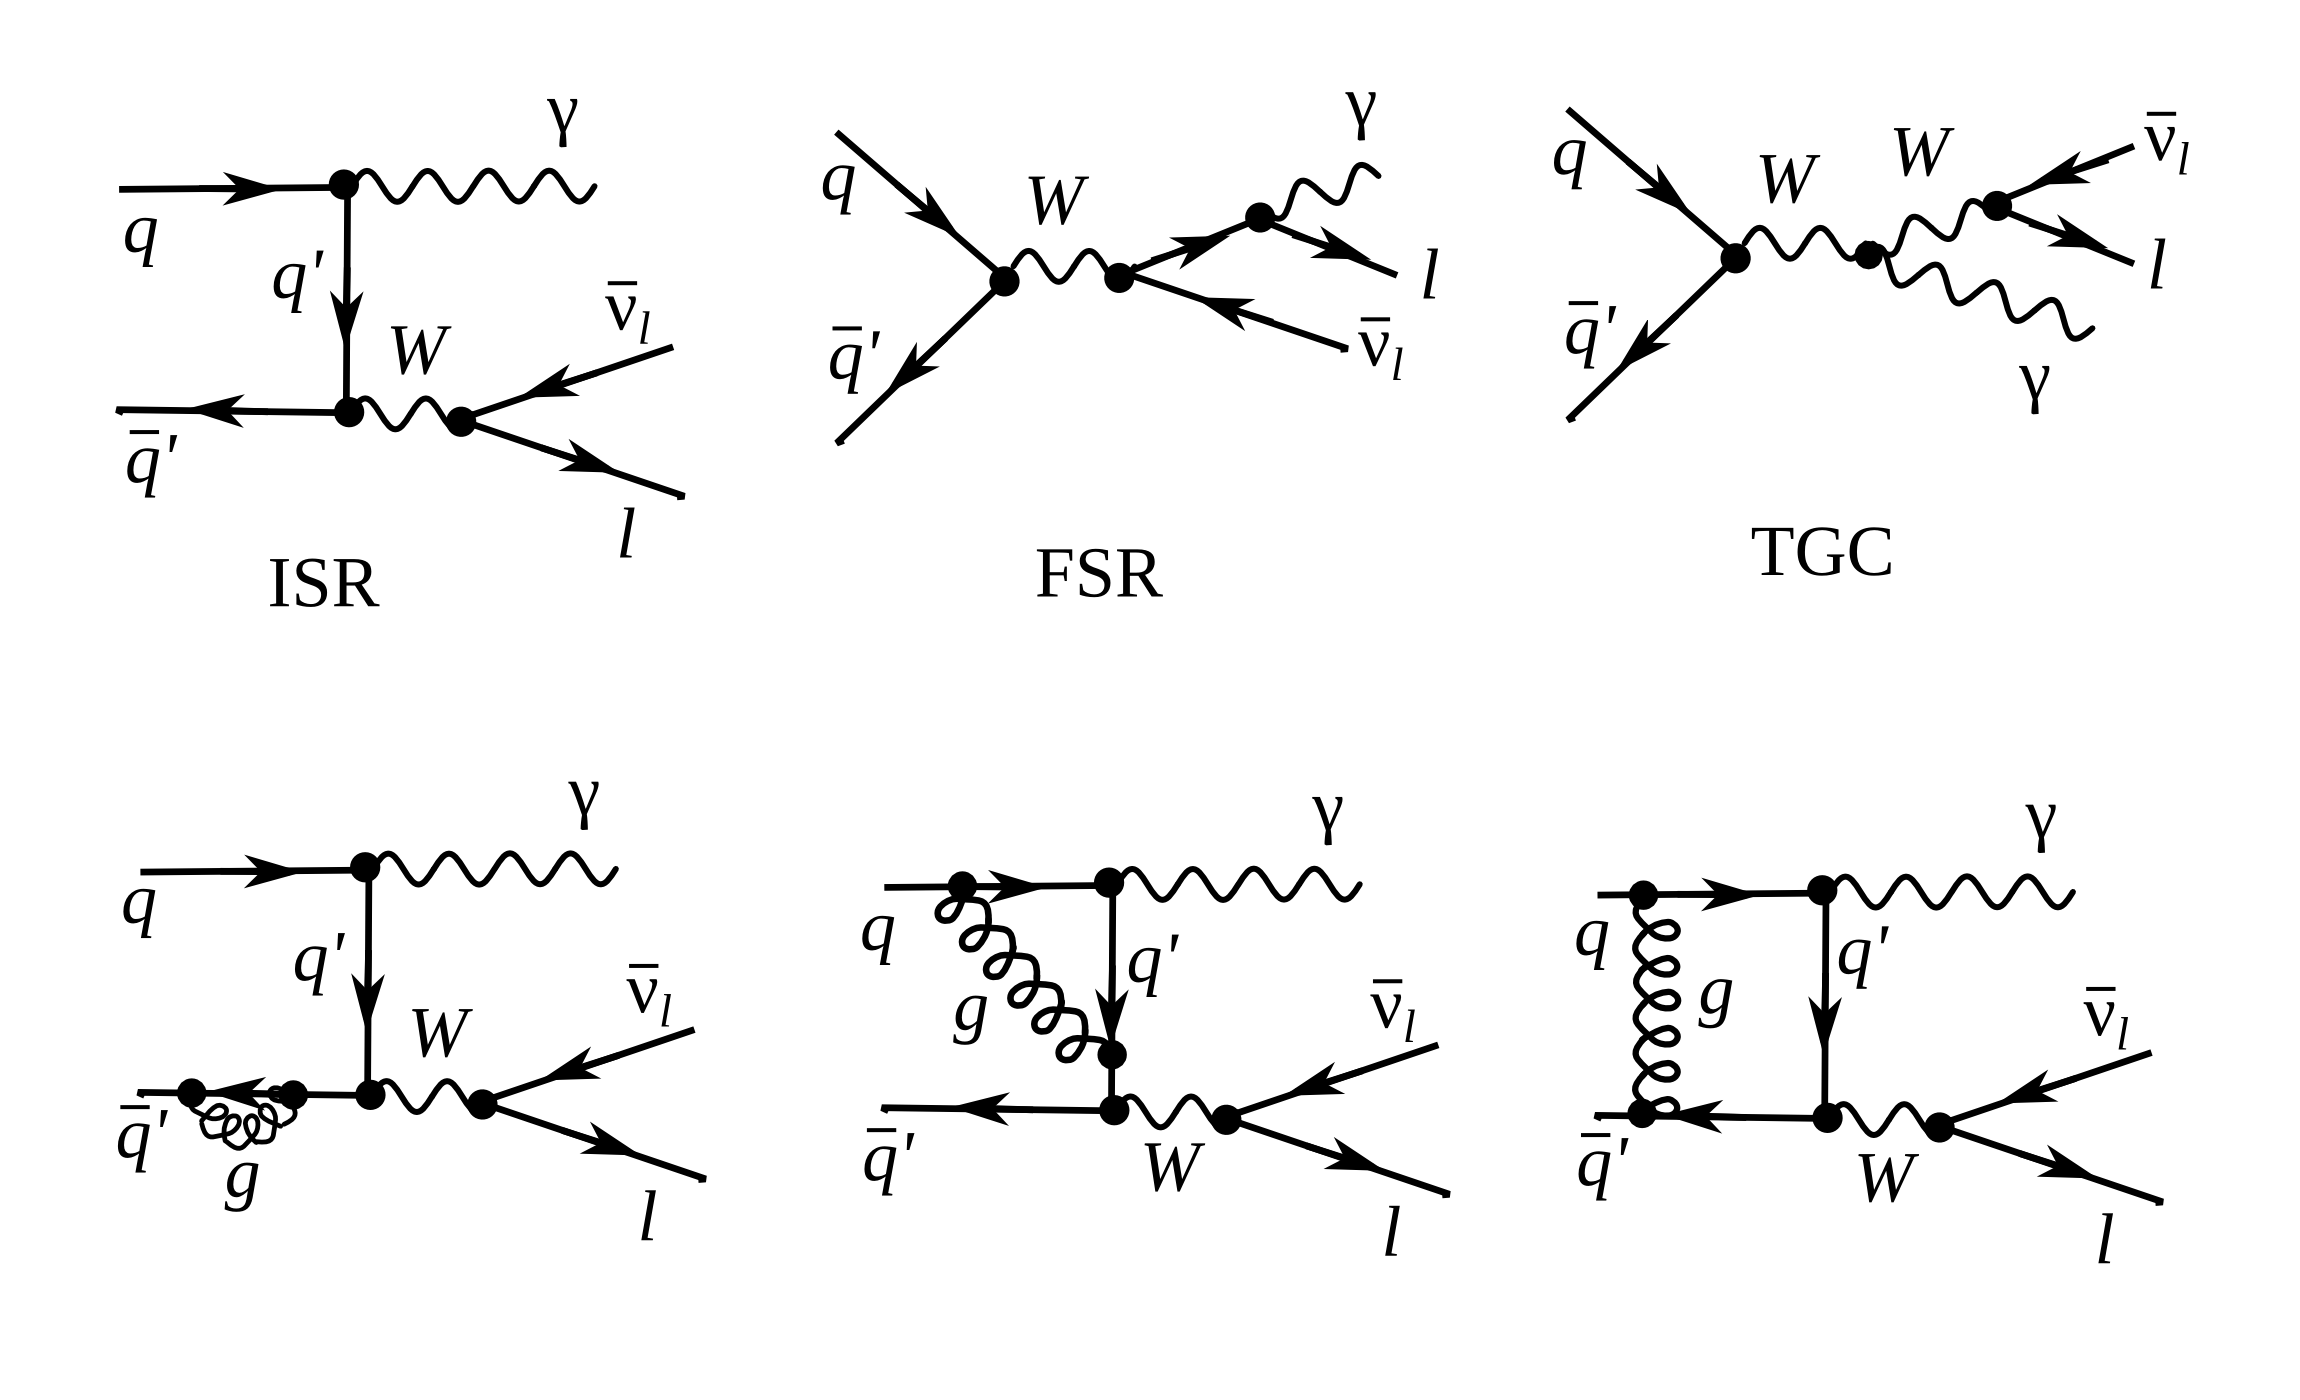
\includegraphics[width=0.90\textwidth]{../figs/WgAbout/feynmWg_LO_NLO.png}}
    \caption{Feynman diagrams of W$\gamma$ production}
    \label{fig:feynmWg_LO_NLO}
  \end{center}
\end{figure}

%Explain Feynman diagrams
%Need Griffiths

%Give a definitions of the total and differential cross section of the Standard Model processes
%Explain LO/NLO/NNLO thing
%Need Griffiths and/or PDG

The cross section of an interaction of two particles can be interppreted as an area around one of the particles which has to be crossed by the other particles so that these two particles would interact. The cross section characterizes the probability of two particles to interact. In the narrower case, the propability of two particles to interact in the exactly way to give a given final state.\\

A number of particles passing through the area $d\sigma$ per unit time is $dN=L \cdot d\sigma$, where L is the luminosity (the number of particles passing through the unit area per unit time). This expression is used to measure the cross section in collision experiments. The actual quantity which can be measured is a number of events of a given process and the luminosity is determined by collider characteristics. L may not be uniform in time however we are usually interested in measuring the total or differential cross section as a function of a certain kinematic paratemeter of a final state particle or of a system of final state particles.\\  
However, to measure the cross section we need to know total number of events of the given process but we cannot detect events which are out of the detector acceptance or which do not fall into the selection criteria we are using in the analysis. Therefore, the bnumber of events $dN$ has to be corrected in a measurement: $dN \rightarrow \frac{dN}{A \cdot \epsilon}$, where $A$ is a detector acceptance and $\epsilon$ is an efficiency of a signal process to pass selection conditions. Other corrections to $dN$ may have to be applied depending on the analysis.\\ 

To compute a cross section theoretically, one has to use Fermi's Golden rule which for the scattering of two particles\\
$1+2\rightarrow 3+4+...+n$\\
has the following form:\\

$\sigma = \frac{S \hbar^2 }{4\sqrt{(p_1p_2)^2-(m_1m_2c^2)^2}} \int |M|^2 (2\pi)^4 \delta^4(p_1+p_2-p_3-p_4-...-p_n) \prod_{j=3}^{n} \frac{1}{2 \sqrt{\bar{p_j^2}+m_j^2 c^2}}\frac{d^3\bar{p_j}}{(2\pi)^3} $\\

To estimate the amplitude $M$, one has to use the Feynman calculus.\\

In case of $W\gamma$, it is the probability of a quark and an antiquark to annihilate with the production of a lepton ($\mu^{\pm}$ or $e^{\pm}$), a neutrino or antineutrino and a photon. The corresponding Feynman diagrams in the LO are shown in Fig. \ref{fig:feynmWg_LO_NLO}, top. 

There are many NLO corrections are possible to these diagrams. QED corrections would mean radiations of extra photons by charged particles, exchange of photons between different charged particles or a photon can be radiated and absorbed by the same charged particle forming a loop. Similarly, weak corrections are possible however they would be much weaker than the QED corrections. But even the QED corrections are too weak compared to QCD corrections which include gluon loops at the same quark line and exchange of a gluon between two different quark lines (Fig. \ref{fig:feynmWg_LO_NLO}, bottom).

%Provide theoretical cross section and order. FSR, ISR, TGC
%Need theory paper
